\documentclass[12pt]{article}
\usepackage{amsmath}
\usepackage{amssymb}
\usepackage{graphicx}
\graphicspath{ {../../Exam_02/} }
\usepackage{tikz}
\usetikzlibrary{trees}
\usepackage[top=1in, bottom=0.75in, left=0.75in, right=0.75in]{geometry}
\newcommand*{\Scale}[2][4]{\scalebox{#1}{\ensuremath{#2}}}%
% \usepackage{showframe}
\usepackage{multicol}
\setlength{\columnsep}{1cm}


\begin{document}
\title{\vspace{-5ex}Math 208 Exam 2: Review for Chapters 5, 7, and 8}
\author{}
\date{\vspace{-5ex}}
\maketitle

\section*{Information}

Exam 2 is on Thursday, March 18, 2021.

\begin{table}[h]
\begin{tabular}{lll}
\hline
\textbf{Section} & \textbf{Time} & \textbf{Submission Deadline}   \\ \hline
Sec 711          & 4:45pm-5:45pm  & 6:05pm \\ \hline
Sec 202          & 6:40pm-7:40pm	& 8:10pm  \\ \hline
\end{tabular}
\end{table}

\subsection*{I have a question about how to do a problem on this study guide}
My email and office hours are posted on canvas. I will also meet with you by appointment. Many of the problems in this study guide have already been solved, either in the homework or during the discussion sections. Both the homework solutions and the discussion notes are posted on Canvas.

\subsection*{Preparing and taking the exam}
\begin{itemize}
\item Arrive early
\item Know how to use your calculator
\item Have extra pencils and an eraser
\item Answer every question (at least minimally)
\item If you get stuck on a question, move on to the next question and come back to it later
\item Double check answers if time allows
\item \textbf{Show your work!}
\end{itemize}

\section*{Chapter 5}

\subsection*{Graphing Inequalities}
Here are some sample problems.
\begin{itemize}
	\item 5.1
	\begin{itemize}
		\item 10: $y > x+1$
		\item 12: $2x-5y \leq10$
		\item 14: $y<5$
		\item p263 Problems 9, 11, 13, 15, 17
	\end{itemize}

% 202
	\item 5.2: p270 Problems 29, 31, 33, 35, 37. Is the region bounded?
	\begin{align*}
		6x+3y\leq 24 \tag{\#32}\\
		3x+6y < 30 \\
		x,y \geq 0
	\end{align*}
	\begin{align*}
		4x+3y\geq 24 \tag{\#34}\\
		3x+4y > 0 \\
		x,y \geq 0
	\end{align*}

% 711
%	\item 5.2: p270 Problems 29, 31, 33, 35, 37. Solve the systems graphically
%\begin{align*}
%	6x+3y\leq 24 \tag{\#32}\\
%	3x+6y < 30 \\
%	x,y \geq 0
%\end{align*}
%\begin{align*}
%	4x+3y\geq 24 \tag{\#34}\\
%	3x+4y > 0 \\
%	x,y \geq 0
%\end{align*}

\item 5.3
\begin{itemize}

% 711
%\item Using the following diagram as a guide, find the corner points of the system of linear inequalities given by 
%\begin{align*}
%	x + y&\le 4 \\
%	2x - y &\le 2 \\
%	x,y \ge 0
%\end{align*}
%\begin{tikzpicture}
%	\draw[black, thick] (-1,0) -- (6,0);
%	\draw[black, thick] (0,-1) -- (0,6);
%	\draw[blue, thick] (0,4) -- (4,0);
%	\draw[red, thick](1,0) -- (4,6);
%	\node at (4.5,-0.5) {$x + y = 4$};
%	\node at (2.5,5.5) {$2x - y = 2$};
%\end{tikzpicture}
%	
%\item The system 
%\begin{align*}
%2x+y &\le 20 \\
%10x+y &\ge 36  \\
%2x+5y &\ge 36 \\
%x &\ge 0  \\
%y &\ge 0  
%\end{align*} 
%has a bounded solution (feasible) region and corner points (3,6), (2,16), (8,4). Minimize $3x +y$ with respect to the system. 
%
%\item The system 
%\begin{eqnarray}
%2x+y &\leq& 20\nonumber \\
%10x+y &\geq& 36 \nonumber \\
%2x+5y &\geq& 36 \nonumber\\
%x &\geq& 0 \nonumber \\
%y &\geq& 0 \nonumber 
%\end{eqnarray} 
%has a bounded solution (feasible) region and corner points (3,6), (2,16), (8,4). Maximize $x +2y$ with respect to the system. 


% 202	
\item \textbf{List} the corner points of the feasible region. \textbf{Maximize and Minimize} the objective function $P=4x+y$. (Make sure to indicate the max and min.) Subject to:
\begin{itemize}
	\item $3x+y \leq 21$
	\item $x+y \leq 9$
	\item $x+3y \le 21$
	\item $x,y \geq 0$
\end{itemize}
\begin{center}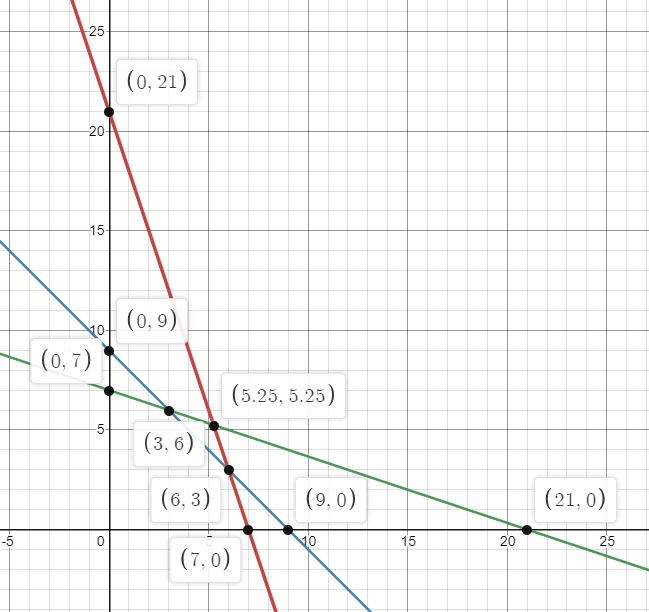
\includegraphics[width=.9\linewidth]{5-2-36}\end{center}


\cleardoublepage
		\item \textbf{List} the corner points of the feasible region. \textbf{Maximize and Minimize} the objective function $P=4x+y$. (Make sure to indicate the max and min.) Subject to:
		\begin{itemize}
			\item $3x+y\geq 15$
			\item $x+y \leq 25$
			\item $x-3y \leq 5$
			\item $x,y \geq 0$
		\end{itemize}
		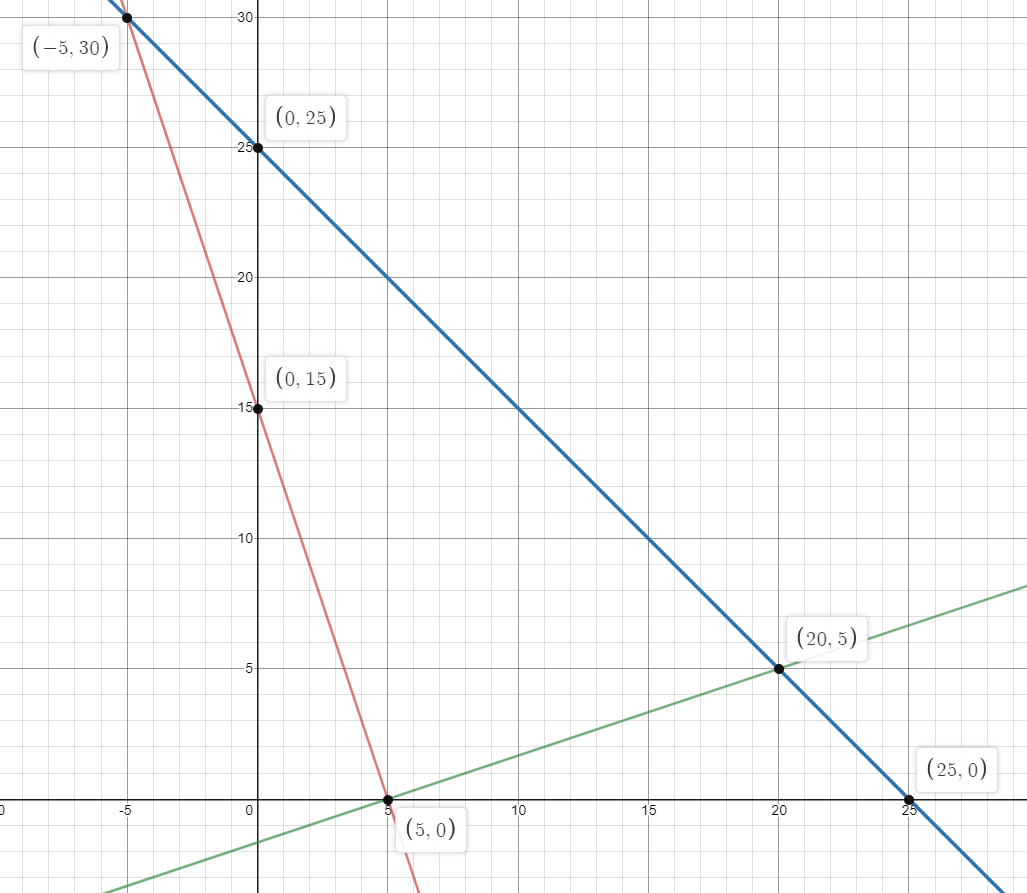
\includegraphics[width=.9\linewidth]{graph}  



% 202
\item \#50: A furniture manufacturing company manufactures dining-room tables and chairs. The relevant manufacturing data are given in the table. \\
\begin{tabular}{|l|r|r|r|}
	\hline
	& \multicolumn{2}{|c|}{Labor hours per unit} & \\
	\hline
	& Table & Chair & Available \\
	\hline
	Assemble & 8 & 2 & 400 \\
	\hline
	Finishing &2 & 1 & 120 \\
	\hline
	Profit per unit & \$90 & \$25 &  \\
	\hline
\end{tabular}
\\\\ Using the  table, \textbf{write the decision variables, objective function, problem constraints, and non-negative constraints}. (Don't solve it!)


\cleardoublepage
\item \#64: A city council voted to conduct a study on inner-city community problems using sociologists and research assistants from a nearby university. Allocation of time and costs per week are given in the table. How many sociologists and how many research assistants should be hired to minimize the cost and meet the weekly labor-hour requirements? What is the minimum weekly cost? \\
\begin{tabular}{|l|r|r|r|}
	\hline
	& \multicolumn{2}{|c|}{Labor hours} & \\
	\hline
	& Sociologist & Research Assistant & Minimum hours per week \\
	\hline
	Fieldwork & 10 & 30 & 180 \\
	\hline
	Research center &30 & 10 & 140 \\
	\hline
	Cost per week & \$500 & \$300 &  \\
	\hline
\end{tabular}
\\\\ Using the  table, \textbf{write the decision variables, objective function, problem constraints, and non-negative constraints}. (Don't solve it!)


\end{itemize}

\end{itemize}


\section*{Chapter 7}
\subsection*{ 7.2: Sets}
\begin{itemize}
	\item Given $U= \{a,b,c,d,e,f,g,h\}, A = \{a,b,e,f\}, B= \{c,d,e,f\},$ and $C= \{g\}$. Find:
	\begin{align*}
		A \cup B &= & A \cap B&=  & A \cap C &= \\
		A' &=  & (A\cup B)' &= & A\cap B' &= 
	\end{align*}
	\item Venn diagrams \\
	\begin{center}
		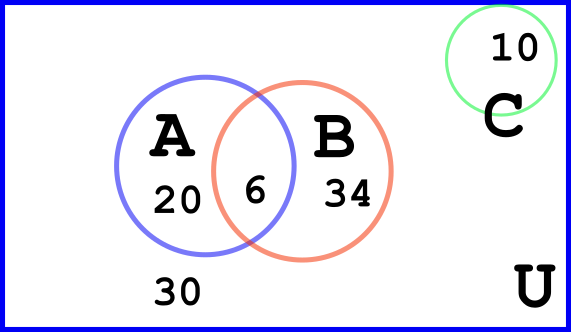
\includegraphics[width=0.5\linewidth]{venn-3}
	\end{center}
	Often, we are interested in how many elements are in a set. This is indicated by $n(A)$. For the above Venn diagram, find:
	\begin{align*}
		n(A) &=   & n(B)&=   & n(C) &=  \\
		n(A \cup B) &=  & n(A \cap B)&=  &n( A \cap C) &=  \\
		n(A') &=  & n(A\cup B)' &=  & n(A\cap B') &= \\
	\end{align*}
\end{itemize}

\subsection*{7.3: Counting}
\begin{align*}
	&n(A\cup B) = n(A) + n(B) - n(A\cap B) &  N_1 * N_2 * \cdots * N_n&
\end{align*}
\begin{itemize}
	\item A survey of 100 families found that 35 families subscribe to the video streaming service Webfilms, 60 families subscribe to the video streaming service Nile Prime, and 20 families subscribe to both video streaming services.
	\begin{enumerate}
		\item How many families subscribe to Webfilms but not Nile Prime?
		\item How many subscribe to Nile Prime but not Webfilms?
		\item How many do not subscribe to either video streaming service?
	\end{enumerate}
	\item An entertainment guide recommends 6 restaurants and 3 plays that appeal to a couple.
	\begin{enumerate}
		\item If the couple goes to dinner or a play, but not both, how many selections are possible?
		\item If the couple goes to dinner and then to a play, how many combined selections are possible?
	\end{enumerate}
\end{itemize}

\subsection*{7.4: $\mathbf{n!, _nP_r, _nC_r}$}
\begin{align*}
	&n! = n(n-1)(n-2)\cdots (2)(1) & n! = n(n-1)!& \\\\
	&_nP_r = \frac{n!}{(n-r)!} & _nC_r = \frac{_nP_r}{r!} = \frac{n!}{r!(n-r)!}&
\end{align*}
Examples:
\begin{align*}
	4! &=  & \frac{8!}{9!} &= \\\\
	\frac{1000!}{999!} &= &  \frac{32!}{4!31!} &= \\\\
	_{30}P_4 &= & _{30}C_4&=
\end{align*}
\begin{itemize}
	\item How many different 5-letter code words can be formed from Q, X, K, V, C, A if no letter is repeated? If letters may be repeated? If adjacent letters must be different?
	\item In a horse race, how many different finishes among the first 3 places are possible if 10 horses are running? (Without replacement)
	
%	711
%	\item From a standard 52 card deck, how many 5-card hands consist of
%	\begin{multicols}{2}
%		\begin{enumerate}
%			\item A$\color{red}\heartsuit$
%			\item Exactly one $\color{red}\heartsuit$
%			\item At least one $\color{red}\heartsuit$
%			\item All $\color{red}\heartsuit$
%		\end{enumerate}
%	\end{multicols}
\end{itemize}


\section*{Chapter 8}

\begin{itemize}
\item \textbf{Basics}
$$\text{Sum of the probability of all possible events (the sample space)}  = 1$$
$$0\leq P(\text{ of any event }) \leq 1$$
\item \textbf{Probability}
$$P(E) = \frac{\text{number of elements in the event}}{\text{number of elements in the sample space}}$$

% 202
\item \textbf{Union Probability}\\

$$P(A \cup B) = P(A) + P(B) - P(A \cap B)$$
$$\text{Disjoint events }P(A \cup B) = P(A) + P(B)$$
\item \textbf{Complement}
$$P(E') = 1-P(E)$$
\end{itemize}

\begin{itemize}
\item What is the sample space of flipping a coin three times?
\begin{itemize}
	\item What is the probability that all three flips will be the same?
	\item What is the probability that all three flips will be different?
	\item What is the probability that the first flip is heads and the last flip is tails?
	\item What is the probability that the first flip is heads or the last flip is tails? 
\end{itemize}

% 202
\item  Suppose that 6 people check their coats in a checkroom. If all claim checks are lost and the 6 coats are randomly returned, what is the probability that all the people will get their own coats back?

\item \textbf{Sample space for rolling two dice}: $S$ is the set of all ordered pairs in the dice chart. What is $n(S)$?
\begin{multicols}{2}
	\begin{enumerate}
		\item $P(sum=7)=$
		\item $P($sum greater than 5$)=$ 
		\item $P($first die is 4$)=$  
		\item $P($sum is prime$)=$ \vfill\null\columnbreak
		\item $P($sum is 7 and sum greater than 5$)=$ 
		\item $P($sum is 7 or sum less than 3$)=$ 
		\item $P($sum is 11)=
		\item $P($sum is 7 or sum is 11)= \vfill\null
	\end{enumerate}
\end{multicols}
\item Given: $P(A)=.4, P(B)=.3, P(C)=.2, P(A\cap B) = .2, P(A\cap C)=0, P(B\cap C)=0$. Find:
\begin{multicols}{2}
	\begin{enumerate}
		\item $P(A\cup B)=$ 
		\item $P(A\cup C)=$ 
		\item $P(A')=$ 
		\item $P(A\cap B \cap C)=$ \vfill\null\columnbreak
		\item $P((A\cap B)')=$ 
		\item $P((B\cap C)')=$ 
		\item $P(B')=$
		\item $P((A\cup B)')=$ \vfill\null
	\end{enumerate}
\end{multicols}


\end{itemize}









\end{document}
